%
% $Id: AttributeSet.java 15 2010-10-11 16:16:32Z justinkamerman $ 
%
% $LastChangedDate: 2010-10-11 13:16:32 -0300 (Mon, 11 Oct 2010) $ 
% 
% $LastChangedBy: justinkamerman $
%

\documentclass[10pt]{report}
\usepackage{graphicx}
\usepackage{setspace}			
\onehalfspacing

\title{CS6999 Programming Assignment 1}
\author{Justin Kamerman 3335272}
\date{\today}

\begin{document}
\maketitle
% No chapter numbers
\renewcommand*\thesection{\arabic{section}}

%----------------------------------------
% Assignment
%----------------------------------------
\section*{Assignment}
\begin{enumerate} 
\item Implement the Aho-Corasick string matching algorithm\cite{RefWorks:103} and test its performance for:
  \begin{itemize}
  \item 1000 blogs and  100 keywords
  \item 2,000 blogs and 100 keywords
  \item 4,000 blogs and 100 keywords
  \item 8,000 blogs and 100 keywords
  \item 16,000 blogs and 100 keywords
  \item 32,000 blogs and 100 keywords
  \end{itemize}
           
Repeat the experiments for 200 and 400 keywords.
      

\item Build an inverted index for 10, 000 blogs. Use 10 keywords to query the index to:
  \begin{itemize}
  \item Locate each keyword and retrieve their corresponding blogs.
  \item Show the intersection of every two keywords. For example, retrieve the document ID of the blogs that keywords 1 and 2 have occurred together at least once. Similarly, for keywords 1 and 3, ..., keywords 2 and 3, keywords 2 and 4, ...
    \item Similarly, show the intersection of every 3 keywords, 4 keywords, etc.
  \end{itemize}
  
\item Do a comparative analysis (time to build the index and time to retrieve) of the two methods.
\end{enumerate}

%----------------------------------------
% Aho-Corasick Algorithm
%----------------------------------------
\section{Aho-Corasick Algorithm}
\label{sec:ahocorasickalgorithm}

\subsection*{Implementation}
The Aho-Corasick algorithm are implemented by a Java
program. The only external dependency is on the Apache commons-cli
library for parsing commend line options. To that end, the program is
operated from the command line, taking options listed in table
~\ref{tab:ahocommandline}.  
\\
\begin{table}[h]
  \centering
  \begin{tabular}{ |l|p{10cm}|} 
    \hline
    Option & Description \\ \hline
    -d          &  Generate Graphviz DOT output. \\ \hline
    -f \<arg\>  &  Path of data file \\ \hline
    -i \<arg\>  &  Number of iterations to perform. Default is 10 \\ \hline
    -n \<arg\>  &  A comma-separated list of attribute names, matching
    the order in which they appear in the data file \\ \hline
    -o \<arg\>  &  Number of folds to create in the training data during. Default is 5. \\ \hline
    -h          &  Print help message \\ \hline
  \end{tabular}
  \caption{Command line options}
  \label{tab:ahocommandline}
\end{table}
\\\\

The program implements various mechanism to facilitate
debugging. Throughout the code, log statements have been added using
the Java logging framework. The logging output is controlled for
individual classes via the \textit{logging.properties} file which the program
read on startup. In addition to logging, code was added to generate
Graphviz DOT (described in ~\cite{RefWorks:110}) output representing
the decision tree created. This output can be rendered using Graphviz
dot tool. An sample dot file for the mushroom.data data set is shown
below. The associated image generated by dot in Figure \ref{fig:dot}.


\begin{verbatim}
digraph G {
	0  [label="0 []", shape=circle];
	0 -> 3 [label="s"];
	0 -> 1 [label="h"];
	1  [label="1 []", shape=circle];
	1 -> 2 [label="e"];
	1 -> 6 [label="i"];
	1 -> 0 [color="red"];
	6  [label="6 []", shape=circle];
	6 -> 7 [label="s"];
	6 -> 0 [color="red"];
	7  [label="7 [his]", shape=circle];
	7 -> 3 [color="red"];
	2  [label="2 [he]", shape=circle];
	2 -> 8 [label="r"];
	2 -> 0 [color="red"];
	8  [label="8 []", shape=circle];
	8 -> 9 [label="s"];
	8 -> 0 [color="red"];
	9  [label="9 [hers]", shape=circle];
	9 -> 3 [color="red"];
	3  [label="3 []", shape=circle];
	3 -> 4 [label="h"];
	3 -> 0 [color="red"];
	4  [label="4 []", shape=circle];
	4 -> 5 [label="e"];
	4 -> 1 [color="red"];
	5  [label="5 [she, he]", shape=circle];
	5 -> 2 [color="red"];
}
\end{verbatim}

\begin{figure}
  \begin{center}
	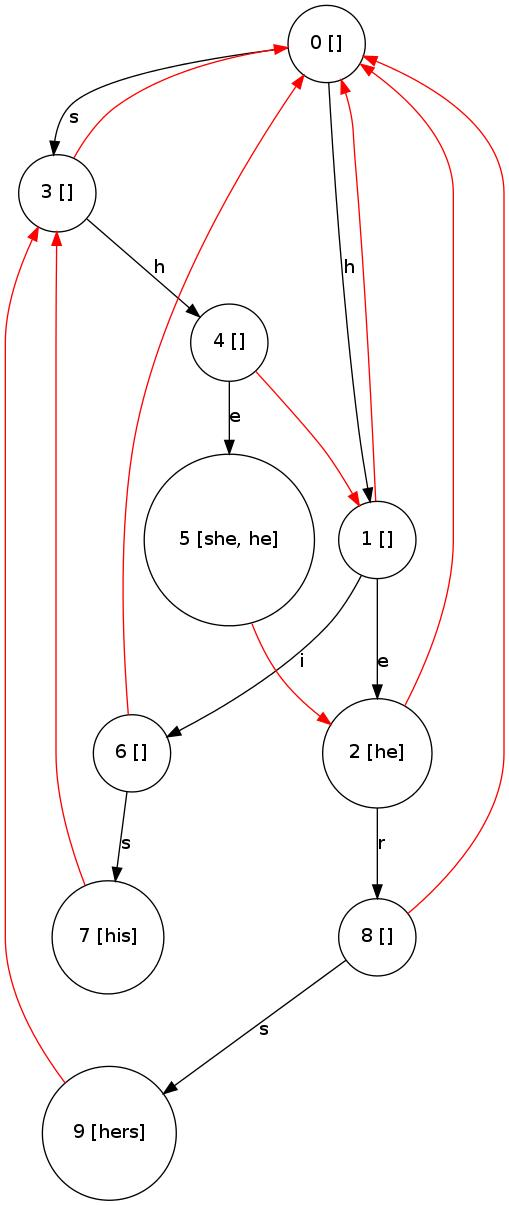
\includegraphics[width=!,height=0.90\textheight]{aho4}
  \end{center}
  \caption{Aho-Corasick state machine visualization generated by DOT}
  \label{fig:dot}
\end{figure} 

\begin{figure}
  \begin{center}
	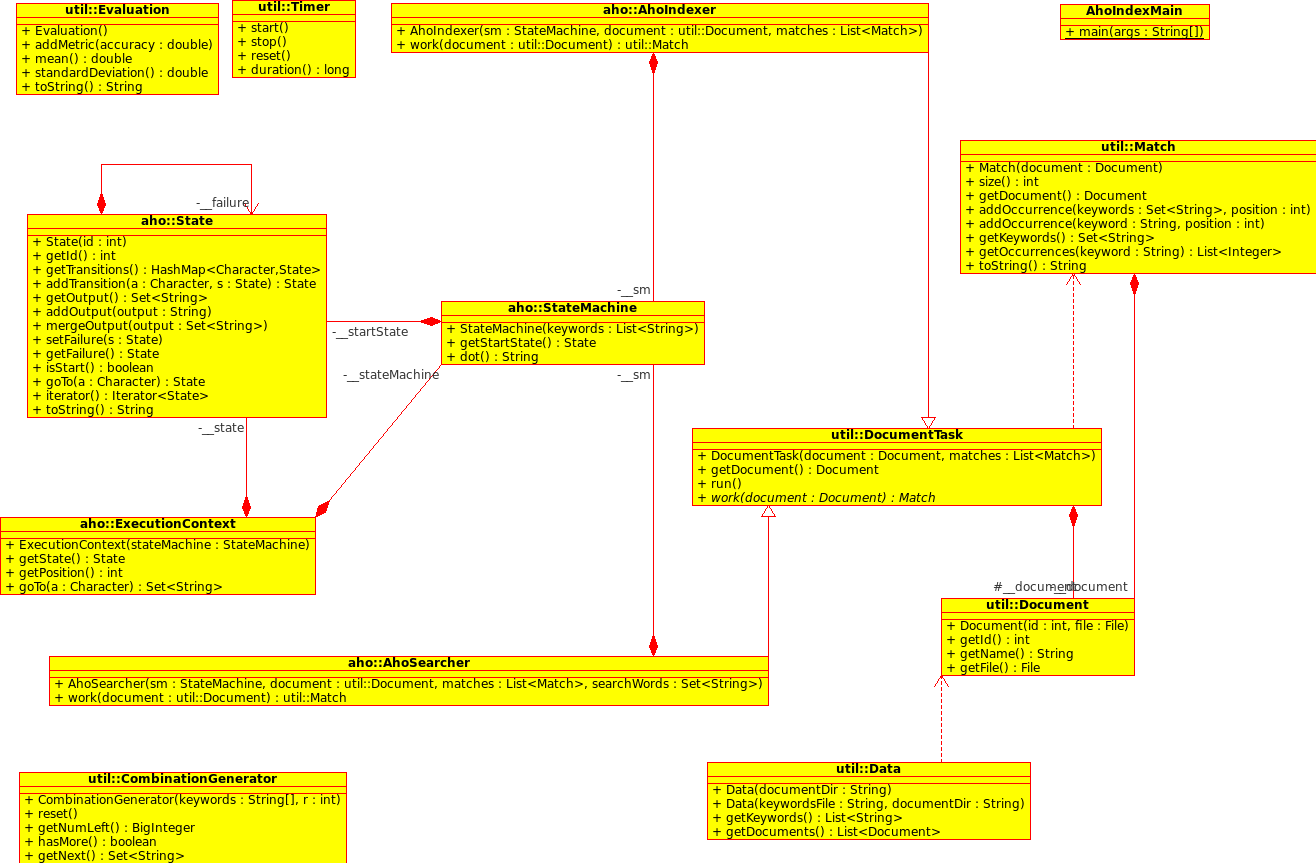
\includegraphics[width=\textwidth,height=!]{ahouml}
  \end{center}
  \caption{Aho-Corasick Implementation UML class diagram}
  \label{fig:ahouml}
\end{figure} 

The implementation classes and their relationships are represented in a UML
class diagram in Figure \ref{fig:ahouml}. Following is a brief
description of each class:

\begin{itemize}
\item \textbf{AhoIndexMain}

\item \textbf{AhoSearchMain} 

\item \textbf{AhoIndexer}

\item \textbf{AhoSearcher} 

\item \textbf{ExecutionContext} 

\item \textbf{StateIterator} 

\item \textbf{StateMachine} 

\item \textbf{Data} 

\item \textbf{Document} 

\item \textbf{DocumentTask} 

\item \textbf{LogFormatter} is a helper class to format log messages.

\item \textbf{Match}

\item \textbf{Timer}

\end{itemize}


%----------------------------------------
% Inverted Index
%----------------------------------------
\section{Inverted Index}
Program expects data in CSV format with attributes occurring first and
classification at the end of each line. All data files have been
preprocessed to fit this format.


\subsection*{Implementation}


\subsection*{Results}



%----------------------------------------
% Algorithm Comparison
%----------------------------------------
\section{Algorithm Comparison}





%----------------------------------------
% Results
%----------------------------------------
\section{Results}
\label{sec:results}
The results of processing each data file using the NBTree
implementation are summarized in Table 
\ref{tab:comparison}. In general, learning time was significantly
higher than both the ID3 and Na\"{i}ve Bayes learning
algorithms. Intuitively, this was expected because of the large number
of Na\"{i}ve Bayes classifiers that are created and evaluated during
the utility calculation.

All tests were run on a personal computer with an AMD Athlon 64 2GHz
Processor, 1GB RAM, running a 32 bit Linux 2.6.31 kernel. The Java
Virtual Machine used was version 1.6.0-18.
\\
\begin{table}[h]
  \centering
  \begin{tabular}{ |l|r|r|r|r|} 
    \hline
    \textbf{Data Set} & \textbf{Na\"{i}ve Bayes} & \textbf{ID3} & \textbf{NBTree 5\%} & \textbf{NBTree 3\%} \\ \hline
    car                      &  0.841449  &  0.938377  & 0.882783  & 0.925797 \\ \hline
    ecoli                    &  0.684776  &  0.384776  & 0.674328  & 0.668657 \\ \hline
    mushroom                 &  0.952007  &  1.000000  & 0.951850  & 0.996921 \\ \hline
    letter-recognition       &  0.737670  &  0.760870  & 0.819500  &          \\ \hline
    breast-cancer-wisconsin  &  0.972662  &  0.945899  & 0.972806  & 0.971223 \\ \hline
  \end{tabular}
  \caption{Comparison of Na\"{i}ve Bayes, ID3, and
    NBTree accuracy over benchmark data sets. NBTree results for both
    3\% and 5\% split utility thresholds are shown}
  \label{tab:comparison}
\end{table}

%----------------------------------------
% Bibliography
%----------------------------------------
\bibliography{bibliography}
\bibliographystyle{IEEEannot}


%--------------------------------------------------
\end{document}
